
\section{Results on LoDoPaB-CT dataset}
% https://latexdraw.com/bar-charts-in-latex-step-by-step-tikz-tutorial/

\begin{frame}{LoDoPaB-CT dataset}
\begin{itemize}
    \item Dataset for low-dose Computed tomography
    \item 35'820 train samples
    \item 3'553 test samples
    \item BM3D as baseline algorithm
    \item Resolution 64 x 64
\end{itemize}

\begin{figure}
    \centering
    \hfill
    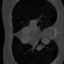
\includegraphics[width=0.16\textwidth]{ct_im_0.png}
    \hfill
    
\includegraphics[width=0.16\textwidth]{ct_im_1.png}
    \hfill
    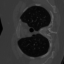
\includegraphics[width=0.16\textwidth]{ct_im_2.png}
    \hfill
    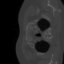
\includegraphics[width=0.16\textwidth]{ct_im_3.png}
    \hfill
    \caption{Some samples from the LoDoPaB-CT dataset.}
  \end{figure}
\end{frame}


\begin{frame}{Evaluation}
\begin{itemize}
    \item Small Scale Experiments
    \begin{itemize}
        \item 1024 train samples
        \item 100 test samples
        \item 200 epochs
        \item<2> \alert{Goal: Find most promising architecture}
    \end{itemize}
    \item Large Scale Experiments
    \begin{itemize}
        \item Complete LoDoPaB-CT dataset
        \item 20 - 40 epochs
        \item<2> \alert{Goal: Find best model}
    \end{itemize}
\end{itemize}
\end{frame}

\begin{frame}{Training}
    \begin{itemize}
        \item U-Net used for reconstruction
        \begin{itemize}
            \item Pre-trained with complete dataset and $SNR_y$ in [-10, 0] for 200 epochs
        \end{itemize}
        \item Mini-batch gradient descent with batch size 64
        \item Adam optimizer
        \item Joint U-Net training possible
    \end{itemize}
\end{frame}

\begin{frame}{Small Scale Results}
    \begin{columns}
        \column{0.5\textwidth}
        \begin{itemize}
            \item Learning fails with random graph
            \item Learning succeeds with defined input graph
            \item Components contribute to success of GAT-Denoiser
            \item Best model with joint U-Net training 
        \end{itemize}
        \column{0.5\textwidth}
        
    \end{columns}
\end{frame}

\begin{frame}{Large Scale Results}
    \begin{figure}
        \centering
        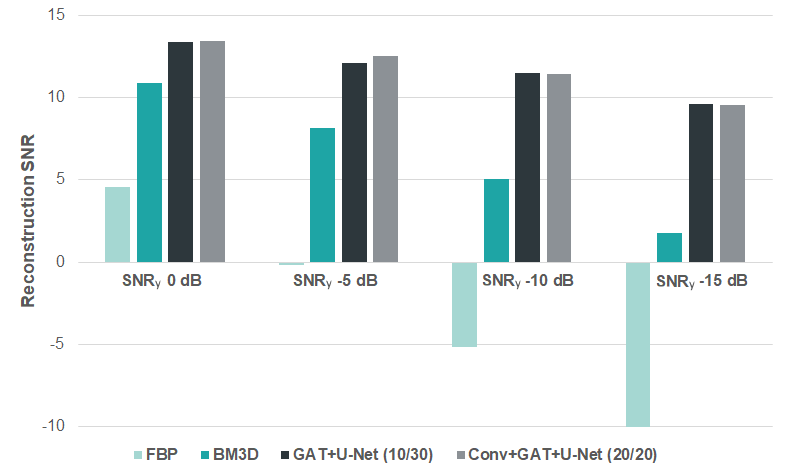
\includegraphics[width=.7\textwidth]{LargeScaleResults.png}
    \end{figure}
\end{frame}

\begin{frame}{Large Scale Results - Visual - $SNR_y$ 0 dB}
\begin{figure}
    \captionsetup[subfigure]{justification=centering}
    \centering
    \begin{subfigure}[t]{0.18\textwidth}
      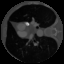
\includegraphics[width=\textwidth]{clean/clean_6.png}
      \caption{Clean sample}
    \end{subfigure} \hfill
    \begin{subfigure}[t]{0.18\textwidth}
      
\includegraphics[width=\textwidth]{fbp/0/fbp_0_6.png}
      \caption{FBP}
    \end{subfigure} \hfill
    \begin{subfigure}[t]{0.18\textwidth}
      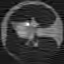
\includegraphics[width=\textwidth]{bm3d_reco/0/bm3d_reco_0_6.png}
      \caption{BM3D}
    \end{subfigure} \hfill
    \begin{subfigure}[t]{0.18\textwidth}
      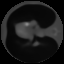
\includegraphics[width=\textwidth]{gat_unet/0/gat_unet_0_6.png}
      \caption{\textit{GAT+U-Net(10/30)}}
    \end{subfigure} \hfill
    \begin{subfigure}[t]{0.18\textwidth}
      
\includegraphics[width=\textwidth]{conv_gat_unet/0/conv_gat_unet_0_6.png}
      \caption{\textit{Conv+GAT+U-Net(20/20)}}
    \end{subfigure} \hfill
    \caption{Large Scale Experiment: Visual results for $SNR_y$ 0 dB.}
  \end{figure}
  

  \begin{tcolorbox}[colback=red!5!white,hide=<1>, alert=<2>, colframe=red!75!black]
    GAT-Denoiser improves BM3D by 27.6\%.
    \end{tcolorbox}
    
\end{frame}


\begin{frame}{Large Scale Results - Visual - $SNR_y$ -10 dB}
    \begin{figure}
        \captionsetup[subfigure]{justification=centering}
        \centering
        \begin{subfigure}[t]{0.18\textwidth}
          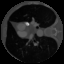
\includegraphics[width=\textwidth]{clean/clean_6.png}
          \caption{Clean sample}
        \end{subfigure} \hfill
        \begin{subfigure}[t]{0.18\textwidth}
          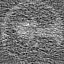
\includegraphics[width=\textwidth]{fbp/-10/fbp_-10_6.png}
          \caption{FBP}
        \end{subfigure} \hfill
        \begin{subfigure}[t]{0.18\textwidth}
          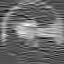
\includegraphics[width=\textwidth]{bm3d_reco/-10/bm3d_reco_-10_6.png}
          \caption{BM3D}
        \end{subfigure} \hfill
        \begin{subfigure}[t]{0.18\textwidth}
          
\includegraphics[width=\textwidth]{gat_unet/-10/gat_unet_-10_6.png}
          \caption{\textit{GAT+U-Net(10/30)}}
        \end{subfigure} \hfill
        \begin{subfigure}[t]{0.18\textwidth}
          
\includegraphics[width=\textwidth]{conv_gat_unet/-10/conv_gat_unet_-10_6.png}
          \caption{\textit{Conv+GAT+U-Net(20/20)}}
        \end{subfigure} \hfill
        \caption{Large Scale Experiment: Visual results for $SNR_y$ -10 dB.}
      \end{figure}
      
    
      \begin{tcolorbox}[colback=red!5!white,hide=<1>, alert=<2>, colframe=red!75!black]
        GAT-Denoiser improves BM3D by 126.0\%.
        \end{tcolorbox}
        
\end{frame}

\begin{frame}{Large Scale Results - Visual - $SNR_y$ -15 dB}
    \begin{figure}
        \captionsetup[subfigure]{justification=centering}
        \centering
        \begin{subfigure}[t]{0.18\textwidth}
          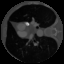
\includegraphics[width=\textwidth]{clean/clean_6.png}
          \caption{Clean sample}
        \end{subfigure} \hfill
        \begin{subfigure}[t]{0.18\textwidth}
          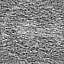
\includegraphics[width=\textwidth]{fbp/-15/fbp_-15_6.png}
          \caption{FBP}
        \end{subfigure} \hfill
        \begin{subfigure}[t]{0.18\textwidth}
          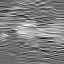
\includegraphics[width=\textwidth]{bm3d_reco/-15/bm3d_reco_-15_6.png}
          \caption{BM3D}
        \end{subfigure} \hfill
        \begin{subfigure}[t]{0.18\textwidth}
          
\includegraphics[width=\textwidth]{gat_unet/-15/gat_unet_-15_6.png}
          \caption{\textit{GAT+U-Net(10/30)}}
        \end{subfigure} \hfill
        \begin{subfigure}[t]{0.18\textwidth}
          
\includegraphics[width=\textwidth]{conv_gat_unet/-15/conv_gat_unet_-15_6.png}
          \caption{\textit{Conv+GAT+U-Net(20/20)}}
        \end{subfigure} \hfill
        \caption{Large Scale Experiment: Visual results for $SNR_y$ -15 dB.}
      \end{figure}
      
    
      \begin{tcolorbox}[colback=red!5!white,hide=<1>, alert=<2>, colframe=red!75!black]
        GAT-Denoiser improves BM3D by 379.9\%.
        \end{tcolorbox}
        
\end{frame}

% \begin{frame}{Some result testing}
%     \begin{tikzpicture}
 
%         \begin{axis} [xbar,bar width=10pt]

%         \addplot[fill = teal] coordinates { (13.34, 3) };
%         \addplot[fill = cyan] coordinates { (13.43, 2) };
%         \addplot[fill = olive] coordinates { (10.85, 1) };
%         \addplot[fill = lime] coordinates { (4.57, 0) };
%         \legend {FBP,BM3D, Conv+GAT+U-Net, GAT+U-Net};
%         \end{axis}
         
%         \end{tikzpicture}
         

% \end{frame}